\chapter[Theoretical Review][Theoretical Review]{Theoretical Review}
\label{chap:standardmodel}

\begin{quote}
  The Standard Model of particle physics is described in brief. It is the preeminent theory describing the behavior of subatomic particles, and it is the result of generations of experimental observations and theoretical interpretations. Until recently, a fundamental particle of the theory had not been observed: the Higgs boson. The particle was first observed by the ATLAS and CMS experiments at the LHC in 2012.
\end{quote}

\section{The Standard Model}

The Standard Model (SM) describes how particles in nature interact in the electroweak and quantum chromodynamic (QCD) sectors. These interactions are encoded in the SM Lagrangian written in the language of a quantum field theory, where particles are represented by quantum fields. The SM Lagrangian is a non-abelian gauge theory with the symmetry group $\text{SU(3)}\times\text{SU(2)}\times\text{U(1)}$. 

The gauge invariance of $\text{SU(3)}$, $\text{SU(2)}$, and $\text{U(1)}$ implies the existent of the eight gluon fields which mediate QCD, the three $W^i$ bosons which mediate the weak sector, and the $B$ boson which mediates the electromagnetic sector, respectively. All of these bosons are predicted to be massless, though, which presents a problem since the weak forces are known to be short range, i.e., their mediating boson ought to be massive.

This problem was remedied independently by Brout and Englert~\cite{1964.Englert.symmetry_breaking}, Higgs~\cite{1964.Higgs.Broken_Symmetries_1,1964.Higgs.Broken_Symmetries_2}, and Guralnik, Hagen, and Kibble~\cite{1964.Guralnik-Hagen-Kibble.symmetry_breaking} in the 1960s. They proposed the symmetry be spontaneously broken by a new scalar field whose accompanying particle has been dubbed the Higgs boson, and the result of this breaking are the massive $W^\pm$ and $Z$ fields, which are superpositions of the massless $W^i$ and $B$ bosons. The symmetry breaking also provides mass terms for the fermions in concert with a Yukawa-style interaction with the Higgs boson. The theory of electromagnetic and weak interactions was coherently unified by Glashow~\cite{1961.Glashow.Partial-symmetries}, Weinberg~\cite{1967.Weinberg.A_model_of_leptons}, and Salam~\cite{1968.Salam.weak-and-EM} in the late 1960s.

Among the first strong evidence for the electroweak theory was the observation of weak neutral current interactions by Gargamelle at CERN~\cite{1973.gargamelle-1,1973.gargamelle-2,1973.gargamelle-3}. These were a manifestation of the massive $Z$ boson despite not having sufficient energy to produce them directly. A handful of additional experiments could also measure the mixing angle $\theta_W$, which is a parameter of the electroweak theory governing the mixing of the $B$ and the $W$ into the $Z$ and photon. This measurement~\cite{1981.weinberg-angle-1,1981.weinberg-angle-2} can be used to make predictions of the masses of the bosons, especially the ratio of their masses: $\text{cos}(\theta_W) = m_W/m_Z$. The UA1 and UA2 experiments at CERN first observed the massive bosons in 1983~\cite{1983.UA1.discovery-of-W,1983.UA1.discovery-of-Z,1983.UA2.discovery-of-W,1983.UA2.discovery-of-Z}, and the measured masses were exactly compatible with the prediction of the broken electroweak symmetry. This provided compelling motivation for the existence of the Higgs boson.

The collection of fundamental SM particles, including the Higgs boson, are shown in \cref{fig:sm-particles-1,fig:sm-particles-2}. The bosons of the SM are mediators of the theory, and the fermions compose the matter we observe. The fermions are grouped into the quarks, which compose objects like protons and neutrons, and the leptons, such as electrons. Quarks have fractional electric charge and three possible color charges, typically called red, blue, and green. They therefore interact with all of the SM gauge bosons. The leptons are colorless and only interact with the electroweak gauge bosons. Among the leptons, neutrinos are electrically neutral and thus only participate in weak interactions. They are also have small mass relative to the other SM fermions, though they are not massless. Understanding the properties of neutrinos is an active area of current research.

\begin{figure}[tp]
  \centering
  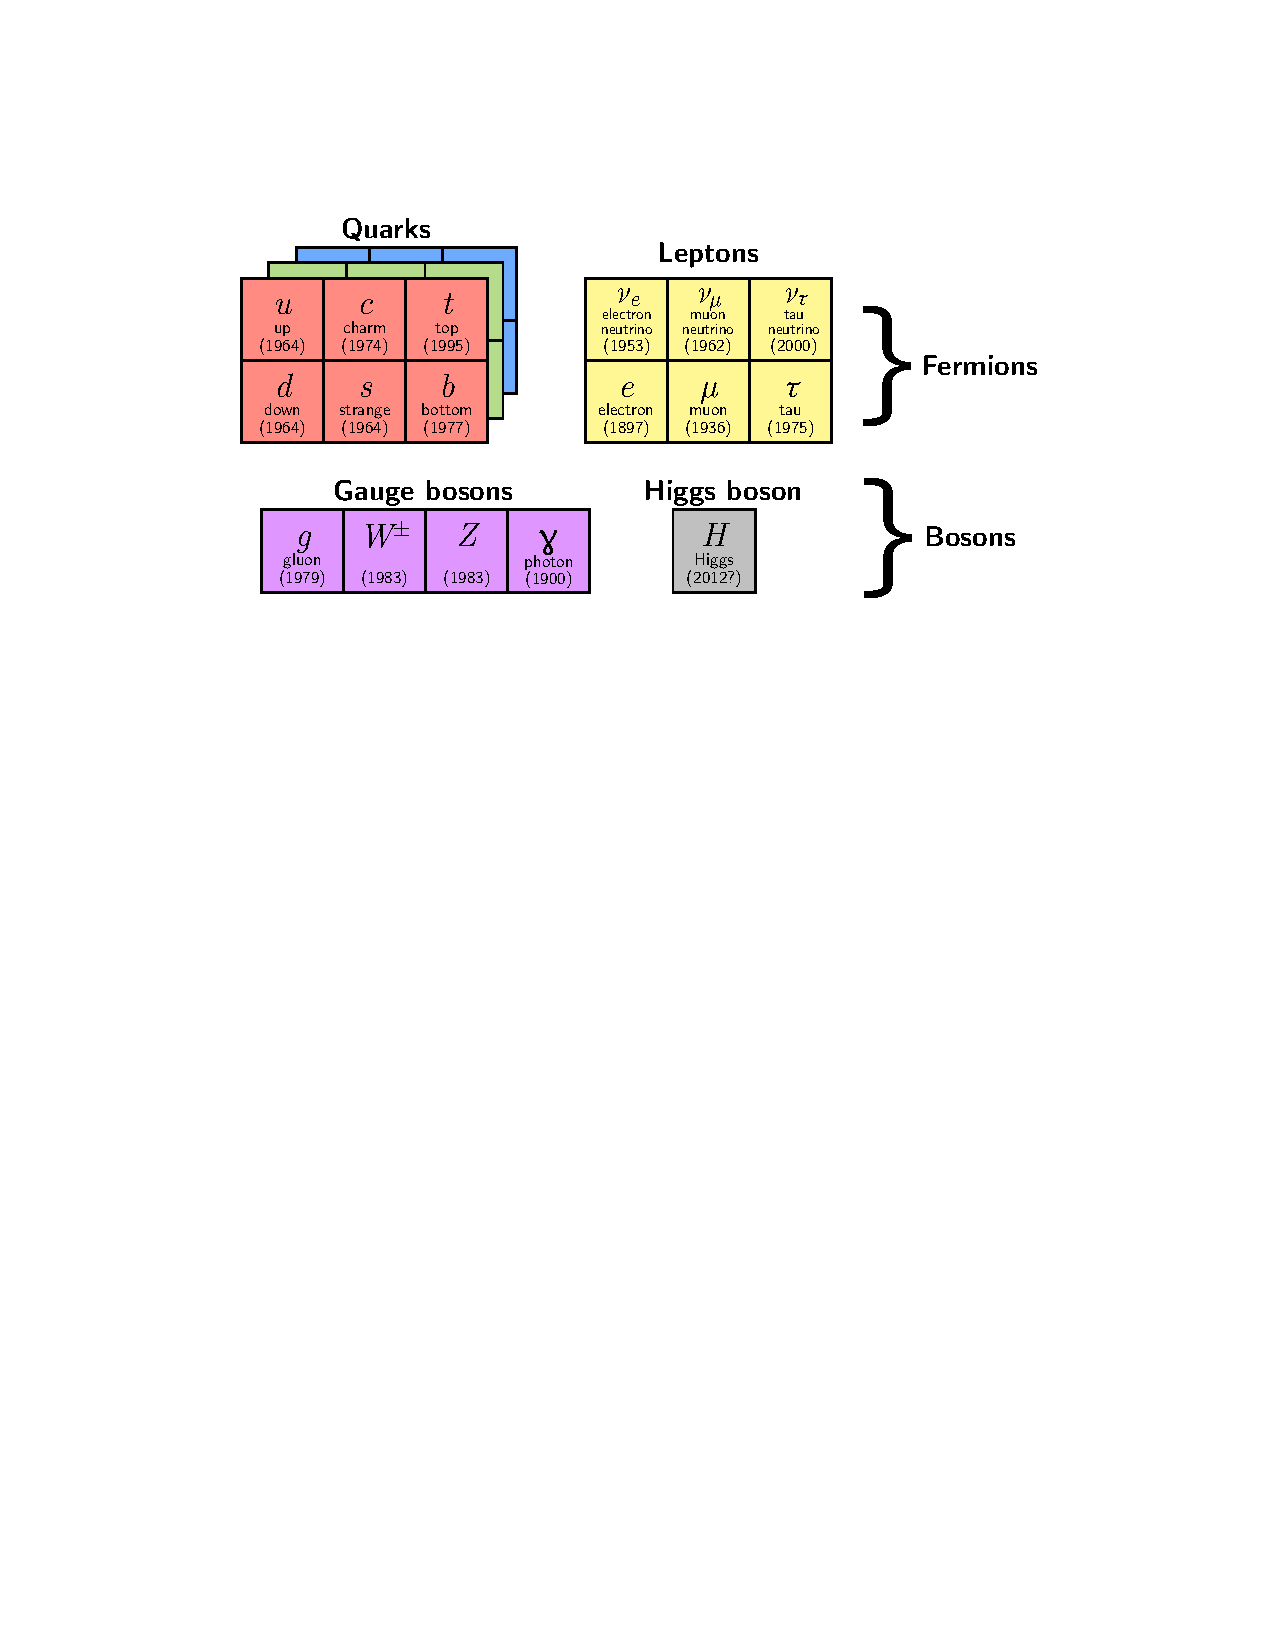
\includegraphics[width=0.95\textwidth]{figures/standardmodel/particles_reece}
  \caption{Simplified illustration of the fundamental particles of the Standard Model~\cite{2013.thesis.ryan}, where the parenthetical note to each particles indicates the year of discovery.}
  \label{fig:sm-particles-1}
\end{figure}

\begin{figure}[tp]
  \centering
  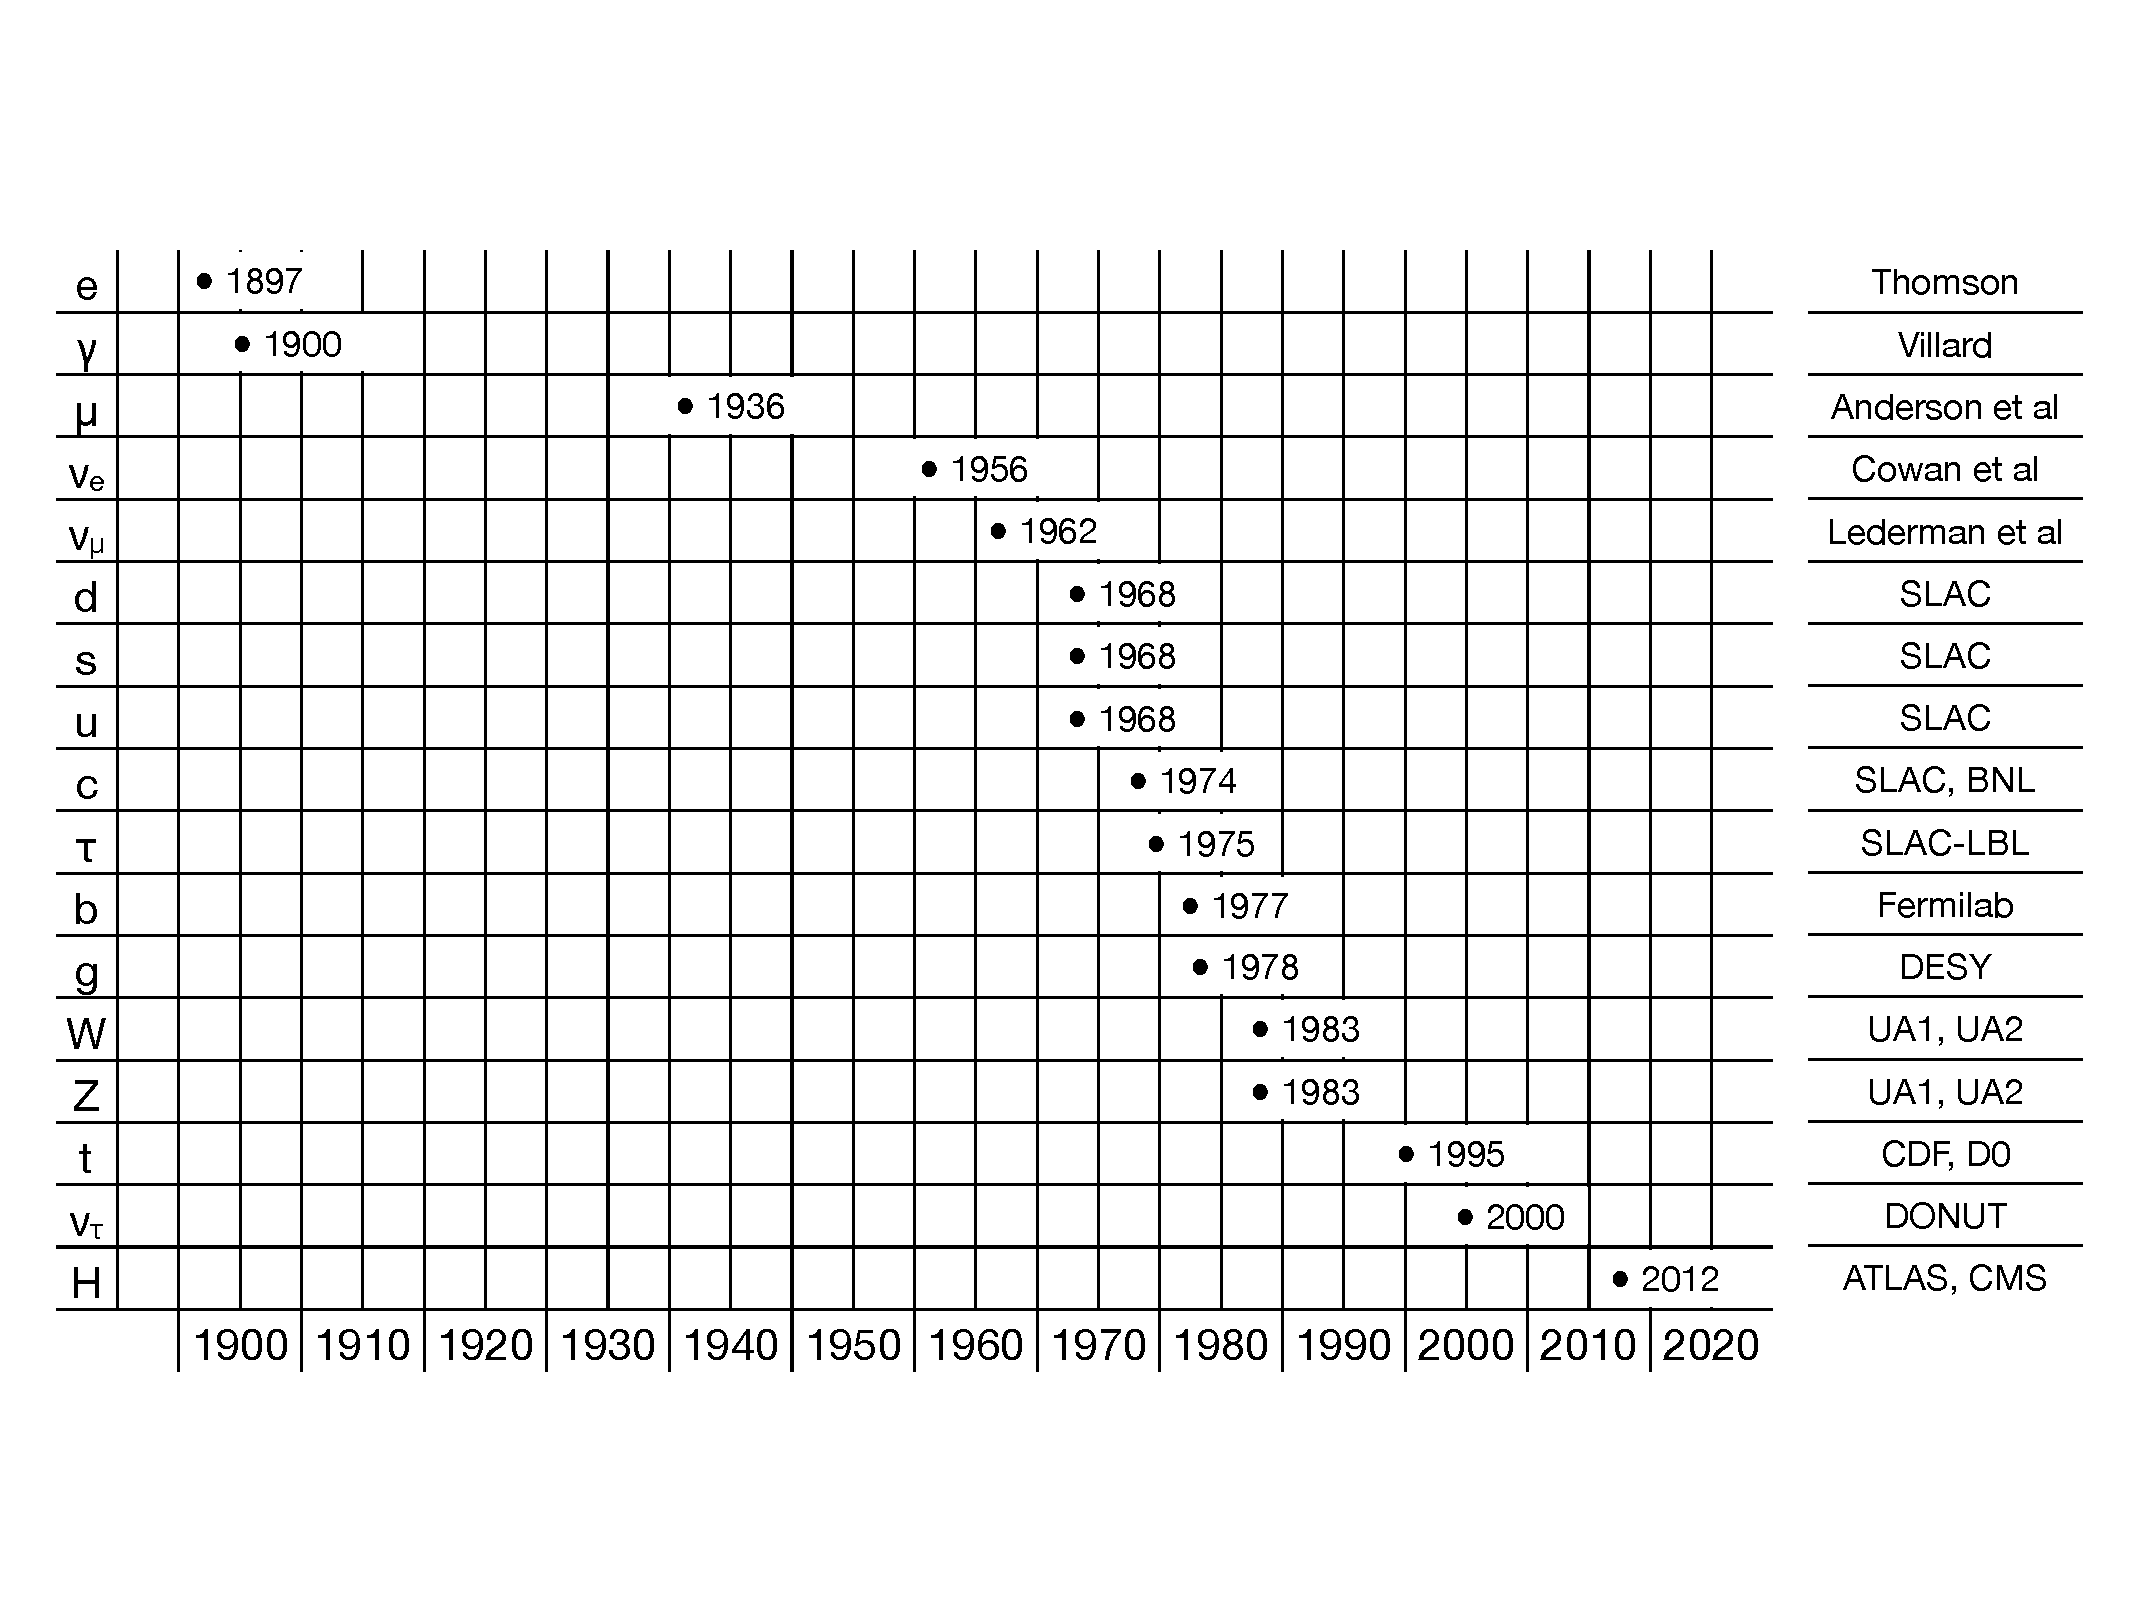
\includegraphics[width=0.95\textwidth]{figures/standardmodel/discoveries}
  \caption{Graph of the discoveries of the fundamental particles of the Standard Model versus time.}
  \label{fig:sm-particles-2}
\end{figure}

\section{Search for the Higgs}

Despite the strong motivation for the existence of the Higgs boson, it was not verified for nearly fifty years after its initial proposal. The topic of experimental observation and general phenomenology of the Higgs boson was approached by Ellis, Gaillard, and Nanopoulos, who decided ``we do not want to encourage big experimental searches for the Higgs boson''~\cite{1976.higgspheno} because its mass was an unknown parameter and its couplings to other particles ``are probably all very small''~\cite{1976.higgspheno}.

Nonetheless, big experimental searches ensued. The largest production modes of the Higgs boson at proton colliders are through gluon fusion (ggF), vector boson fusion (VBF), and production in association with a vector boson ($VH$)~\cite{1984.vbf}, and the cross-sections for these processes are indeed small. The diagrams are shown in \cref{fig:sm-higgs-diagrams} with their cross-section for the Higgs mass at 125 GeV. At electron colliders, the $ZH$ production mode dominates. 

The Higgs then decays quickly, and experiments are tasked with inferring its presence from its decay products. Many decay channels are allowed because the Higgs couples directly to all massive particles in the SM Lagrangian. The Higgs decay branching fractions~\cite{1997.hdecay} are correlated with the mass of the decay products, and it tends to decay to whatever particle is heaviest and kinematically allowed. For example, if the Higgs mass was 100 GeV, it would decay almost exclusively to $bb$, whereas at 200 GeV, it would decay mostly to $WW$ and $ZZ$.

\begin{figure}[tp]
  \centering
  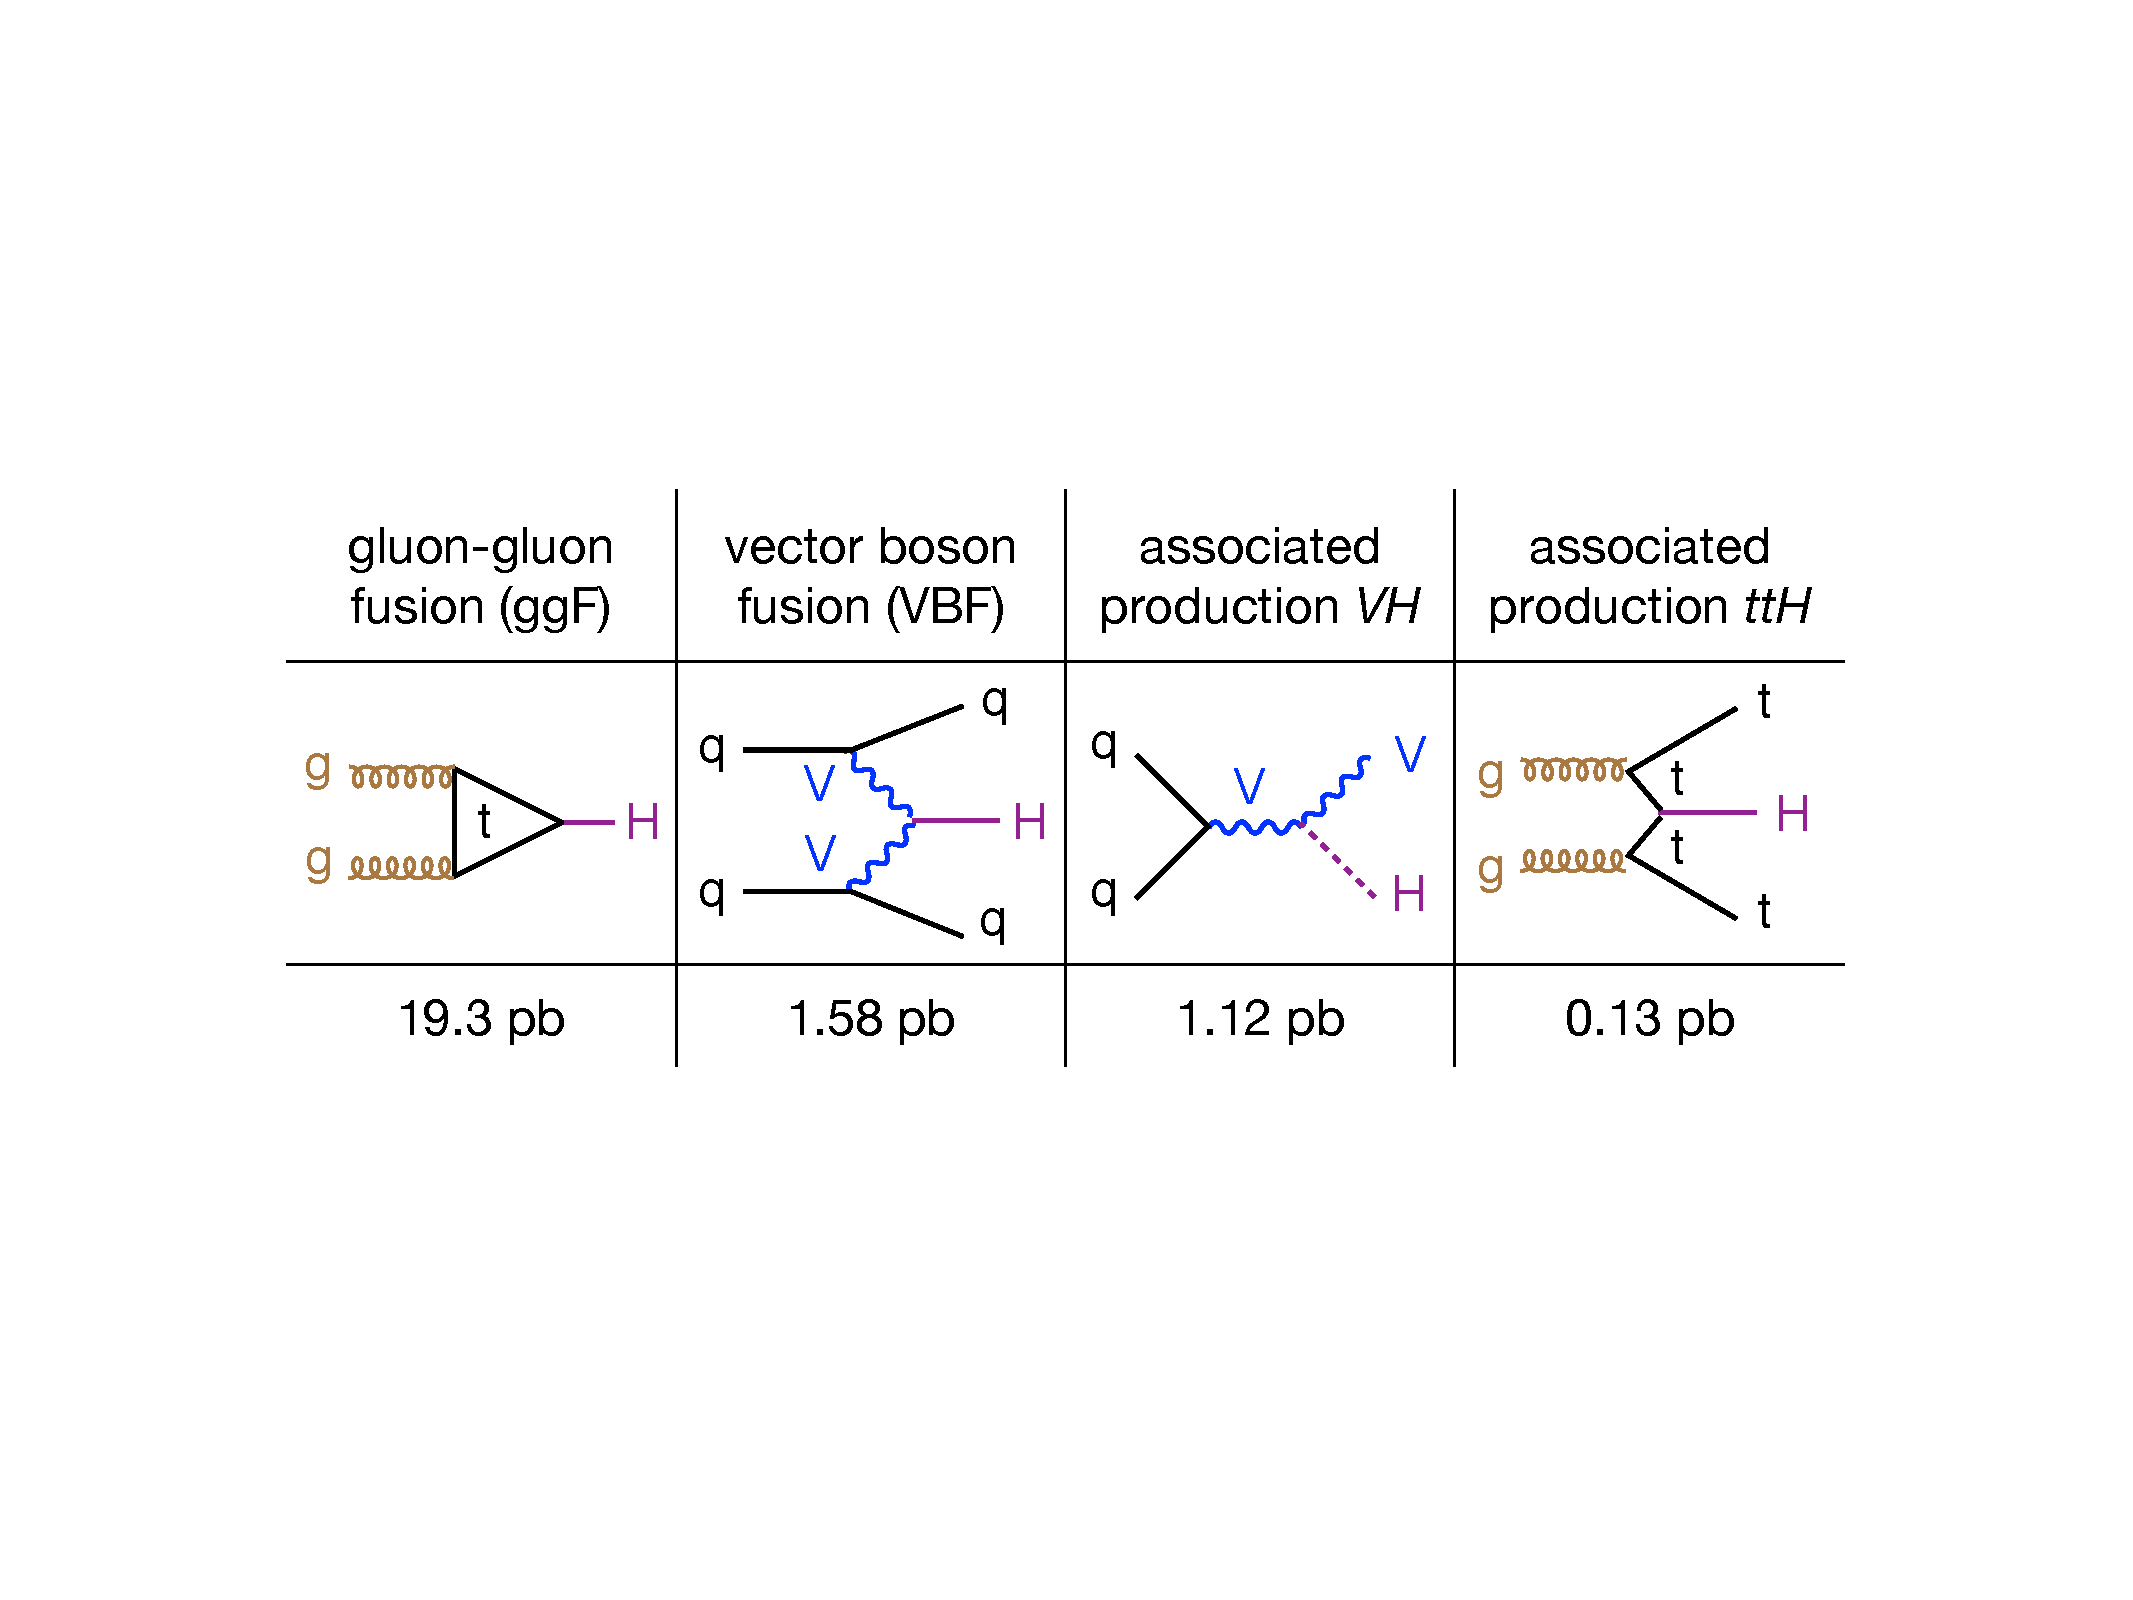
\includegraphics[width=0.95\textwidth]{figures/standardmodel/higgsproductions}
  \caption{Selected Higgs boson production mechanisms and their cross-sections at $pp$ colliders with $\sqrt{s} = 8$ TeV for $m_H \!=\! 125$ GeV~\cite{2013.lhchxswg}.}
  \label{fig:sm-higgs-diagrams}
\end{figure}

The prospect of directly observing the Higgs boson was a major piece of the physics program at the LEP~\cite{1996.cern-press} and Tevatron~\cite{2001.fermilab-press} colliders at CERN and Fermilab, respectively. Experiments at both colliders published many searches~\cite{2003.lep-higgs,2013.tevatron-higgs}, and their sensitivity was driven by the $\Hbb$ decay channel because of its high branching fraction. Neither collider reported an observation, and the LEP experiments excluded SM production of the Higgs boson if its mass were below 114 GeV.

The LEP and Tevatron searches, when combined with fits of precision electroweak measurements sensitive to the mass of the Higgs boson, showed a preference for the Higgs boson mass to be between 115 and 200 GeV, as shown in \cref{fig:sm-gfitter}. This set the stage for the ATLAS and CMS experiments at the LHC, with a collision energy much higher than the Tevatron, to finally observe or exclude the existence of the Higgs boson in the first few years of data-taking.

\begin{figure}[tp]
  \centering
  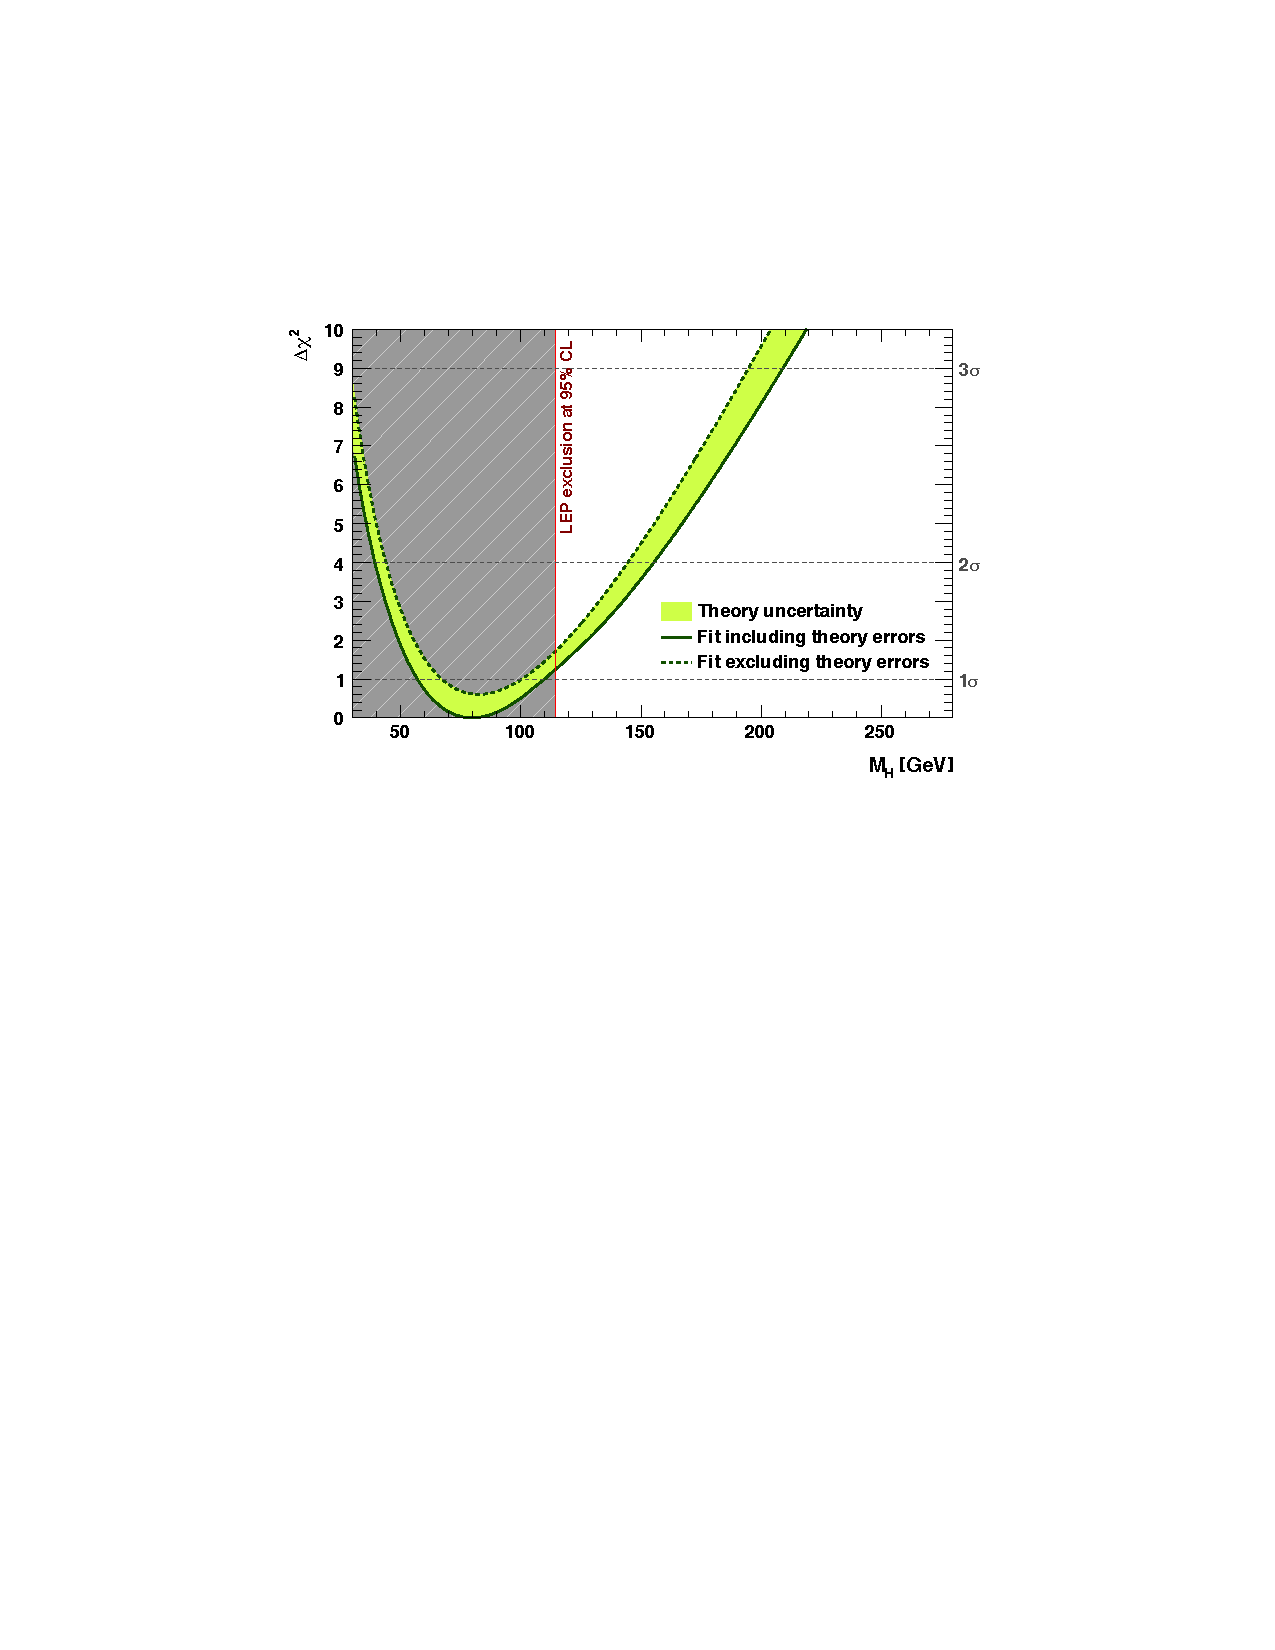
\includegraphics[width=0.48\textwidth]{figures/standardmodel/gfitter_standardfit}
  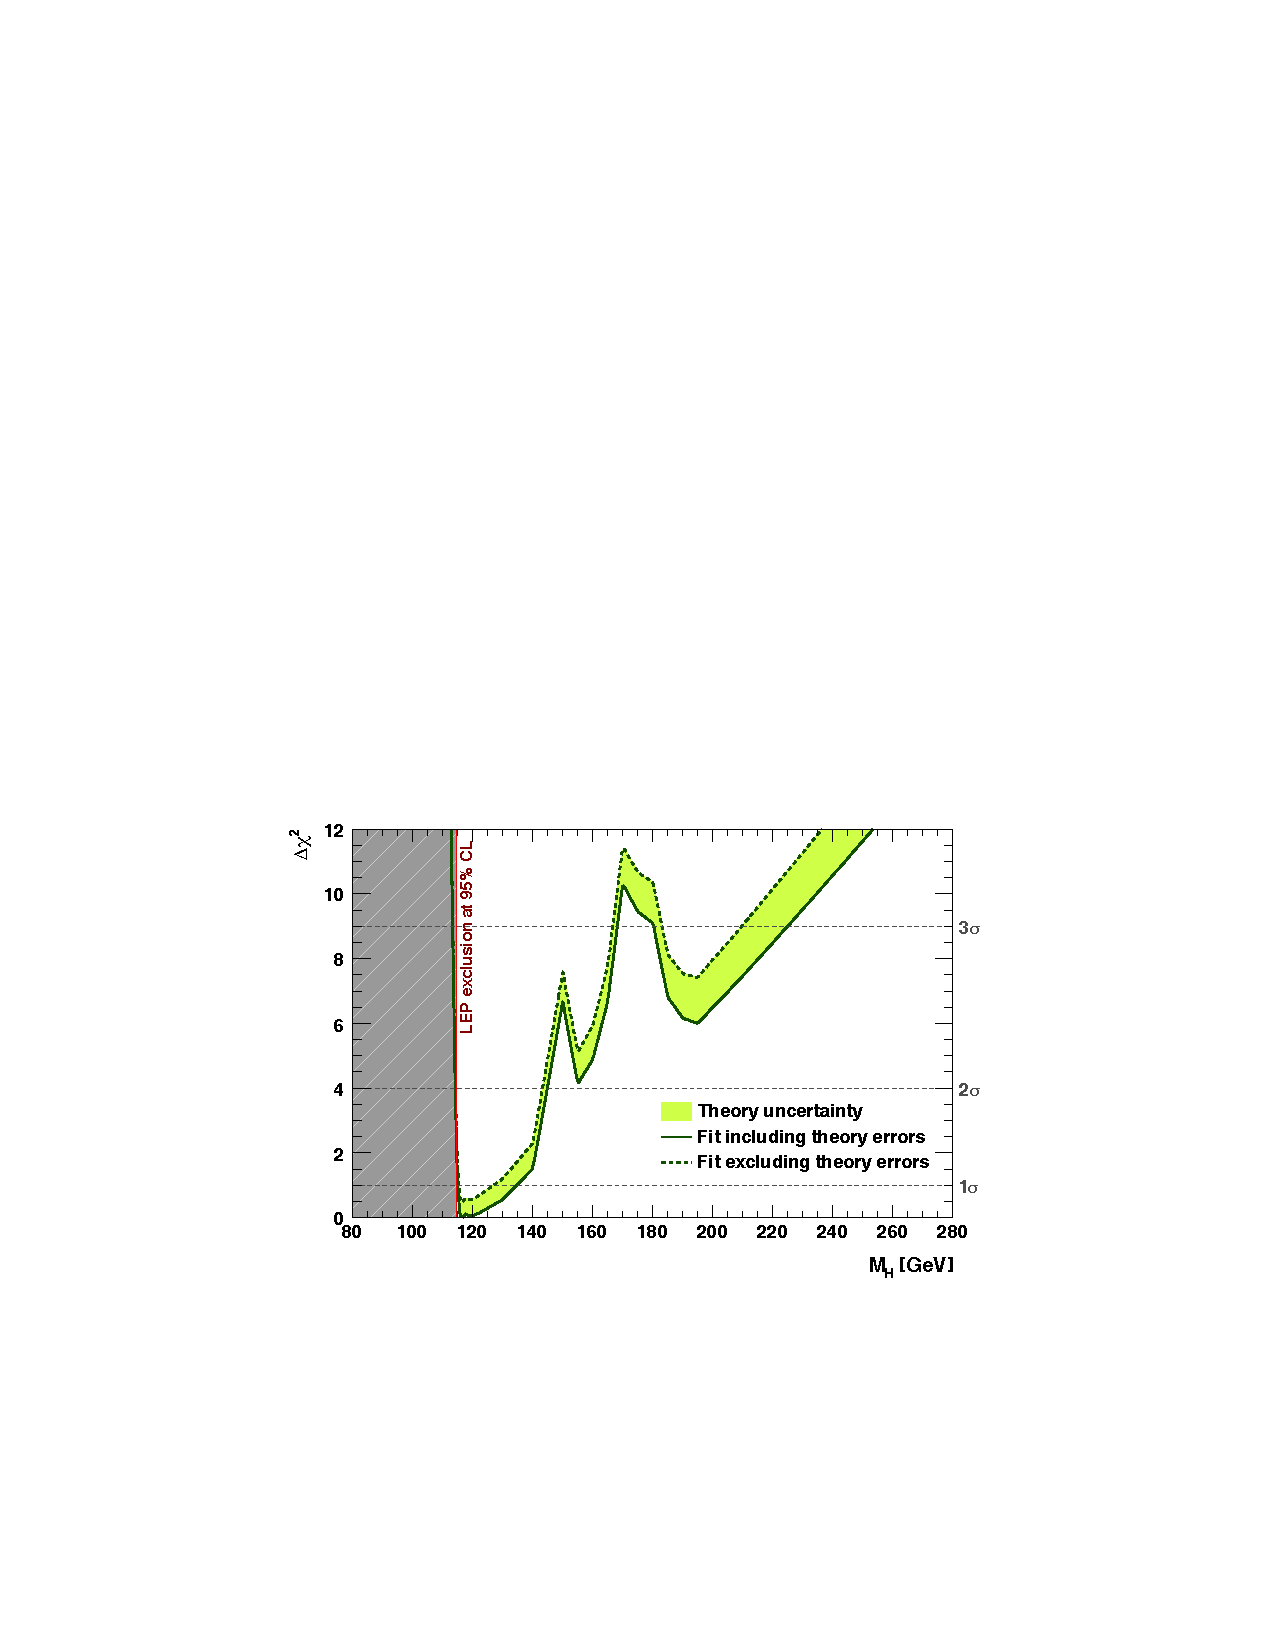
\includegraphics[width=0.48\textwidth]{figures/standardmodel/gfitter_completefit}
  \caption{Summary of the preferences for the Higgs mass as a result of global fits to precision electroweak data~\cite{2009.gfitter} without direct Higgs searches from LEP and the Tevatron (left) and with (right). The fits are done before LHC data-taking.}
  \label{fig:sm-gfitter}
\end{figure}

The ATLAS and CMS experiments independently announced the observation of the Higgs boson in 2012~\cite{HIGG-2012-27,2012.cms-higgs}, using data taken with proton collisions at 7 and 8 TeV. The measured mass was around 125 GeV, consistent with expectations from global electroweak fits and the LEP and Tevatron exclusions. The discovery was driven by the bosonic decay modes: $\Hyy$, $\HZZ$, and $\HWW$. ATLAS and CMS have only recently unearthed evidence for the fermionic decay modes, driven by the $\tautau$ channel, and that is the topic of this thesis.

Two Nobel prizes in physics have been awarded for the theory of electroweak symmetry breaking~\cite{nobelprizes}. Glashow, Salam, and Weinberg were honored in 1979 for the unified theory of electroweak symmetry breaking after the observation of neutral current interactions at Gargamelle. Englert and Higgs were honored in 2013 for the introduction of spontaneous symmetry breaking after the observation of the Higgs boson at ATLAS and CMS.

\section{Shortcomings}

The Standard Model beautifully describes particles physics across many orders of magnitude and in both the electroweak and QCD sectors. However, it is not a complete theory of the universe. There are many aspects of the physical universe for which the SM provides an unsatisfactory description, or no description at all. These are among the strongest reasons for continuing to search for physics beyond the SM. The upcoming years of data-taking at the LHC hope to push the boundaries of our understanding, and to shed light in these uncertain areas.

\begin{description}

    \item[Dark matter, dark energy] \hfill \\
      Astrophysical experiments in the past decades~\cite{2006.darkmatter,2013.planck} have indicated that only around 5\% of the universe is composed of observable matter, like protons and electrons. The origin and properties of the remaining 95\% are largely unknown. The remainder is generally put into two groups: dark matter, which seems clumped and localized, and dark energy, which seems to permeate all space. Neither dark matter nor dark energy is incorporated into the SM.

    \item[Gravity] \hfill \\
      Gravity is the force which dictates the movement of stars and planets, and keeps humans from floating into space. It is completely missing from the SM. A particle mediating gravity, called the \textit{graviton}, is hypothesized and could probably be accommodated into the SM. But there is no observation of such a particle yet or any experimentally motivated descriptions of its interactions with the rest of the SM particles.

    \item[Hierarchy and Unification] \hfill \\
      Nature has so far displayed two fundamental energy scales: the electroweak scale of the Standard Model ($10^{2}$ GeV), and the Planck scale where the effect of gravity on particle interactions cannot be ignored ($10^{18}$ GeV)~\cite{1998.hierarchy}. Why are these energy scales are separated by sixteen orders of magnitude, and what physics exists between them? The SM offers no motivation for these disparate scales, nor does it offer an elegant unification of the fundamental forces. Many popular models of physics beyond the SM, such as supersymmetry, offer more satisfactory descriptions of the high energy regimes~\cite{1997.susyprimer}.

\end{description}

